\documentclass[11pt]{article}
\usepackage[margin=1in]{geometry}
\usepackage{amsmath,amssymb}
\usepackage{graphicx,float}
\usepackage{subcaption}
\usepackage{xcolor}
\usepackage{tikz}
\usetikzlibrary{arrows.meta, positioning}
\usepackage{booktabs}
\usepackage{enumitem}
\usepackage[colorlinks=true, linkcolor=blue!50!black, citecolor=blue!50!black]{hyperref}

\title{\textbf{Learning Transformations Between Breast-Phantom Volumes with Flow Matching}\\[4pt]
\large From a Failed Interpolation Attempt to a Validated 180\textdegree{} Rotation Task}
\author{Daniel Kozin \\ \small ID 215550260 \\ \small Diffusion Models, Course Project}
\date{}

\begin{document}
\maketitle
\vspace{-0.6cm}

\begin{abstract}
We train a flow-matching model over a dataset of 3D breast-phantom voxel volumes and use it
for two tasks. The first, our original goal, is to interpolate between two real phantoms by
inverting each to the model's noise space, blending there, and integrating forward. This
approach produces excellent single-phantom reconstructions but unreliable interpolations:
generated volumes either collapse onto one endpoint or tear into disconnected anatomy, a
failure that persists across more training, a class-weighted loss, more integration steps, and
a partial-inversion variant of the method. We trace this to a structural property of flow
matching rather than a bug: with no compression bottleneck, nothing in training constrains the
region between two different real phantoms' noise pre-images. We then pivot to a
self-supervised task with exact ground truth, predicting a phantom rotated $180^\circ$,
which lets us iterate against a known-correct answer instead of visual judgment alone. A
sequence of diagnosed failures (an undercommitted velocity field, an over-permissive
cross-entropy term, and finally exposure bias between teacher-forced training and the model's
own multi-step rollout) leads to a rollout-consistency loss that raises combined mask Dice from
$0.13$ to $0.453 \pm 0.151$ on 176 held-out validation pairs, with no evidence of overfitting.
\end{abstract}

\section{Introduction}
Flow-matching and diffusion models learn a transformation from a simple noise distribution to
a complex data distribution by regressing a velocity field along straight-line paths between
paired noise and data samples. Beyond generation, an appealing use of such a model is
\emph{editing}: if the noise space the model has learned is smooth and well-organized, moving
along a path between two real data points there should decode into a smooth, meaningful
sequence of anatomy in between them, rather than the physically meaningless blur a direct
voxel-space crossfade would produce. This project set out to test that idea on a dataset of 3D
breast-phantom volumes: invert two real phantoms into the model's noise space, interpolate, and
generate the volume in between. That attempt did not work, for reasons that turn out to be
informative about what flow matching does and does not guarantee. We diagnose the failure, then
pivot to a task the model \emph{can} be trained and evaluated on with exact ground truth,
predicting a $180^\circ$ rotation of a phantom, and report the sequence of loss and
evaluation fixes that took that second task from a model that never moves its prediction at all
to one with a validated combined mask Dice of $0.453$.

In summary, this paper:
\begin{itemize}[noitemsep]
\item documents why an inversion-slerp-integration approach to phantom interpolation fails, and
traces the failure to the absence of a compression bottleneck in flow matching rather than to a
correctable implementation error;
\item introduces and evaluates a partial-inversion variant of that approach, showing that it
narrows \emph{where} the model breaks down without fixing \emph{why};
\item reformulates the underlying problem as a self-supervised $180^\circ$ rotation task with an
exact, closed-form target, removing the need to judge success by eye alone;
\item develops, through a sequence of diagnosed failures, a rollout-consistency loss that raises
validated combined mask Dice from $0.13$ to $0.453\pm0.151$ on 176 held-out pairs, with no
evidence of overfitting.
\end{itemize}

\section{Background: Flow Matching}
We have a data distribution we can sample from but have no formula for (real phantoms,
one-hot encoded over the 4 classes so each voxel becomes a length-4 vector), and a distribution
we understand completely, standard Gaussian noise $x_0\sim\mathcal N(0,I)$ of the same shape.
Writing a data sample as $x_1$, the simplest path between the two is a straight line,
\begin{equation}
x_t = (1-t)\,x_0 + t\,x_1, \qquad t\in[0,1], \label{eq:path}
\end{equation}
whose velocity is constant along the path: $\tfrac{d x_t}{dt} = x_1 - x_0 =: v^*$. A network
$v_\theta(x,t)$ is trained to predict this velocity at randomly sampled points along randomly
sampled paths,
\begin{equation}
\mathcal{L}(\theta) = \mathbb{E}_{t\sim U[0,1],\,x_0\sim\mathcal N(0,I),\,x_1\sim p_{\text{data}}}
\Big[\, \|v_\theta(x_t,t) - (x_1-x_0)\|^2 \,\Big]. \label{eq:loss}
\end{equation}
Generation integrates this field forward from noise; Euler's method with $n$ steps of size
$\Delta t = 1/n$ repeats
\begin{equation}
x_{t+\Delta t} = x_t + v_\theta(x_t,t)\,\Delta t, \label{eq:euler-fwd}
\end{equation}
from $x_0$ at $t=0$ to a generated $\hat x_1$ at $t=1$; taking the class-wise argmax turns the
continuous output back into a discrete label volume. The same field also runs backward: given a
real $x_1$, integrating
\begin{equation}
x_{t-\Delta t} = x_t - v_\theta(x_t,t)\,\Delta t \label{eq:euler-bwd}
\end{equation}
from $t=1$ to $t=0$ recovers an approximate noise pre-image $\hat x_0$, i.e.\ \emph{inversion}.

\section{Data}
Each phantom is a 3D voxel volume ($26$ depth slices $\times\,128\times128$), with every voxel
labeled as one of four classes: background, insert (the overall phantom surface), pillar
(holding the lump in place), or lump, the class that matters medically, and the rarest one.
After removing double/triple-lump phantoms (out of scope for this single-lump framing), 123
files across 40 case IDs remain, expanded to 984 volumes via $8\times$ in-plane rotation
augmentation. Figure~\ref{fig:dataset} shows four examples, and Table~\ref{tab:balance} gives
the measured class balance: the two classes that matter, pillar and lump, together make up
barely one percent of every volume. This imbalance shapes several of the design and diagnosis
decisions throughout the paper.

\begin{figure}[H]
    \centering
    \begin{subfigure}[b]{0.22\textwidth}
        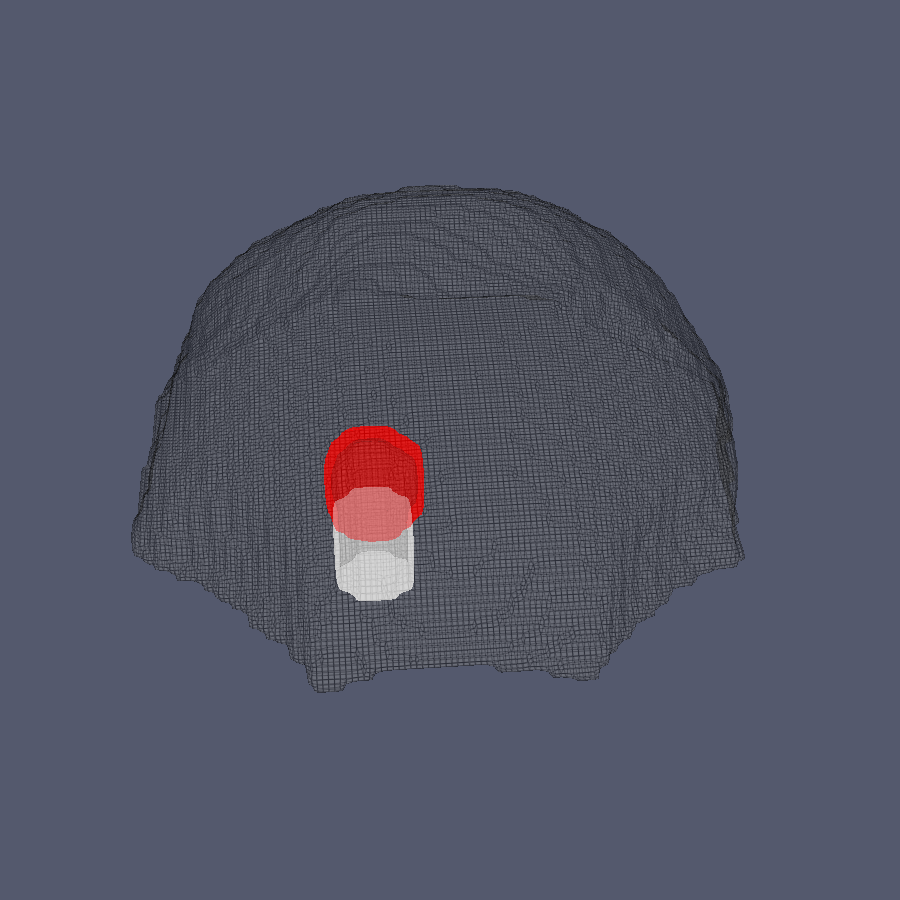
\includegraphics[width=\textwidth]{imgs/showcase_showcase_gt_0.png}
    \end{subfigure}
    \hspace{1em}
    \begin{subfigure}[b]{0.22\textwidth}
        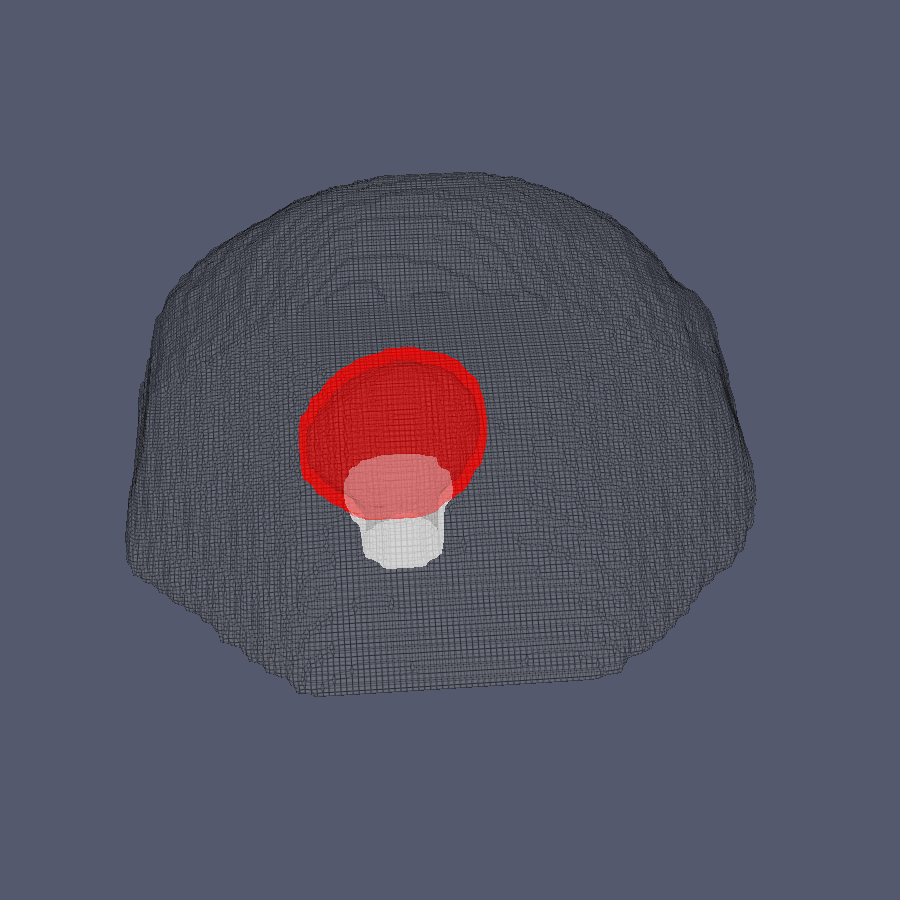
\includegraphics[width=\textwidth]{imgs/showcase_showcase_gt_13.png}
    \end{subfigure}
    \hspace{1em}
    \begin{subfigure}[b]{0.22\textwidth}
        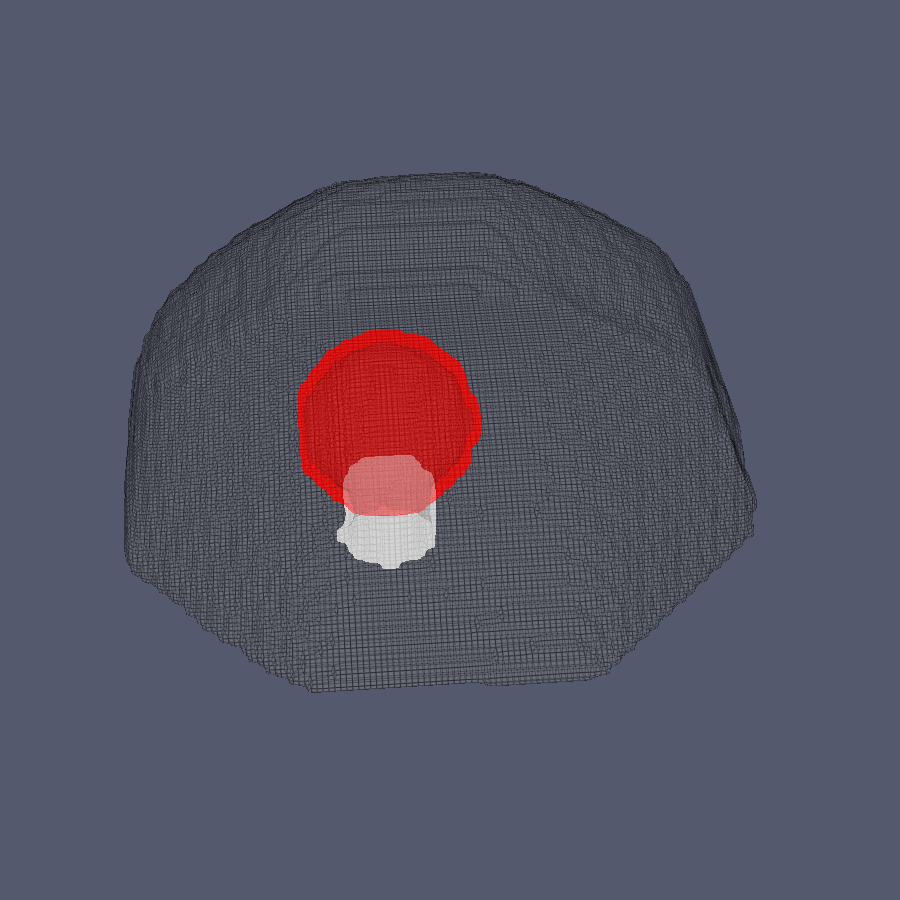
\includegraphics[width=\textwidth]{imgs/showcase_showcase_gt_70.png}
    \end{subfigure}
    \hspace{1em}
    \begin{subfigure}[b]{0.22\textwidth}
        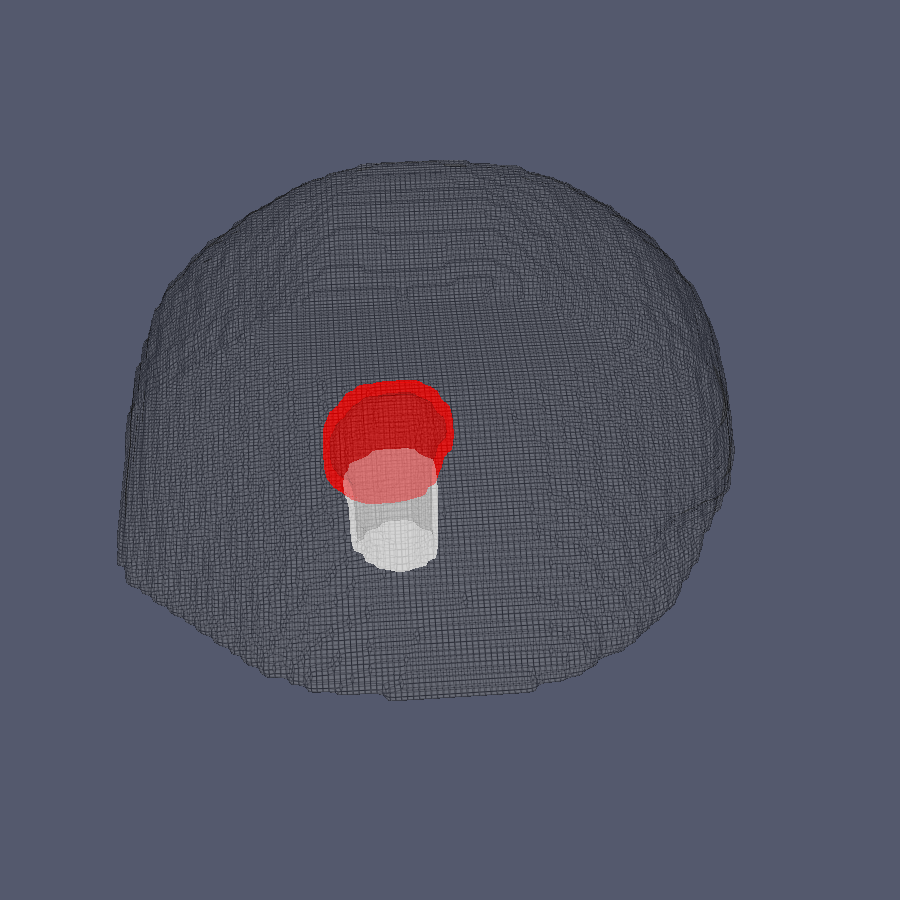
\includegraphics[width=\textwidth]{imgs/showcase_showcase_pred_8.png}
    \end{subfigure}
    \caption{Examples from the breast-phantom dataset. Gray is the phantom surface, red is the
    lump, and white is the pillar holding the lump.}
    \label{fig:dataset}
\end{figure}

\begin{table}[H]
\centering
\begin{tabular}{@{}lcccc@{}}
\toprule
Class & Background & Insert & Pillar & Lump \\
\midrule
Voxel share & 50.8\% & 48.0\% & 0.32\% & 0.94\% \\
\bottomrule
\end{tabular}
\caption{Measured voxel class balance across the dataset.}
\label{tab:balance}
\end{table}

\section{Noise-Space Interpolation Between Real Phantoms}

\subsection{Method overview}
To morph between two real phantoms A and B, we invert both to noise ($\hat x_0^A, \hat
x_0^B$), interpolate between the two noise representations at mixing fraction $\alpha\in[0,1]$,
and integrate the result forward through $v_\theta$ back to a label volume
(Figure~\ref{fig:pipeline}).

\begin{figure}[H]
    \centering
    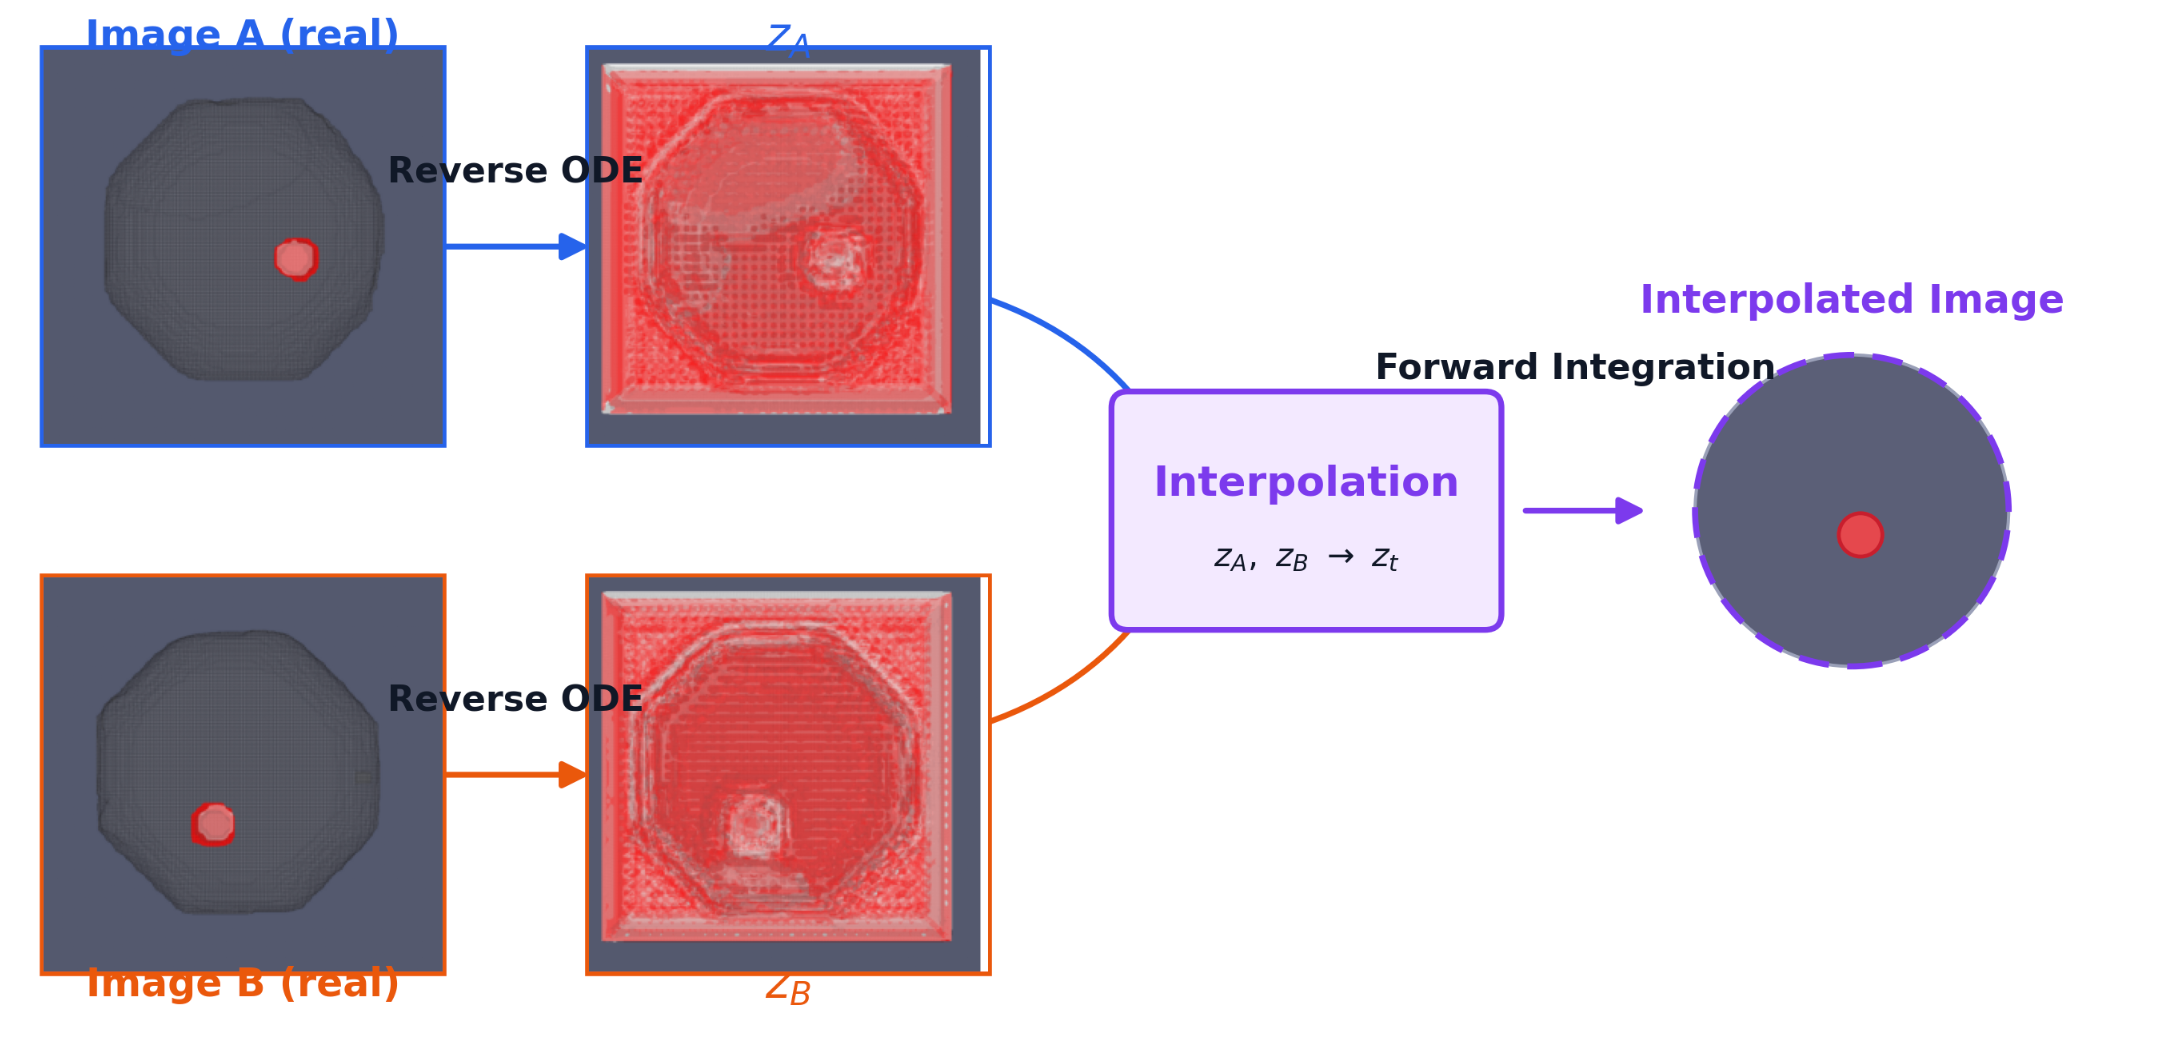
\includegraphics[width=\textwidth]{imgs/pres/pipeline.png}
    \caption{The interpolation pipeline: both real phantoms are inverted to noise, combined,
    and integrated forward through the learned velocity field.}
    \label{fig:pipeline}
\end{figure}

\subsection{Spherical interpolation}
A plain linear blend of two Gaussian noise vectors is the wrong operation: in a space of
dimension $d\approx 1.7\times10^6$ (four channels $\times$ 26 $\times$ 128 $\times$ 128), two
independent Gaussian samples concentrate tightly around a shell of radius $\sqrt d$, while their
average has expected norm only $\sqrt{d/2}\approx 0.71\sqrt d$, since two independent, essentially
orthogonal random directions of equal length shrink when averaged, the same way two arrows in a
narrow "V" shrink at their midpoint. This handily quantifies why a linear blend hands the
network a point from a region of space it never trained on. Spherical interpolation (slerp)
avoids this: it moves along the great-circle arc between the two points instead of stepping
through the interior, preserving their common norm exactly at every mixing fraction,
\begin{equation}
\mathrm{slerp}(a,b,\alpha) = \frac{\sin\big((1-\alpha)\theta\big)}{\sin\theta}\,a +
\frac{\sin(\alpha\theta)}{\sin\theta}\,b, \qquad
\theta=\arccos\!\left(\frac{a\cdot b}{\|a\|\|b\|}\right). \label{eq:slerp}
\end{equation}
The full pipeline per $\alpha$ is therefore: invert A and B, slerp between $\hat x_0^A$ and
$\hat x_0^B$ at that $\alpha$, integrate forward, argmax, render.

\subsection{Class-weighted loss}
Because background and insert dominate the voxel count (Table~\ref{tab:balance}), plain,
unweighted MSE (Eq.~\ref{eq:loss}) can be driven close to zero while the model is essentially
wrong about the lump. We weight the per-voxel error by class,
\begin{equation}
\mathcal{L}_{\text{weighted}}(\theta) = \mathbb{E}\left[\frac{1}{C\!\cdot\!D}
\sum_{c=1}^{C} w_c \sum_{\text{voxels}} \big(v_\theta - v^*\big)^2_{c,\text{voxel}}\right],
\label{eq:weighted-loss}
\end{equation}
with weights set to the square root of inverse class frequency (to avoid a handful of rare
voxels dominating the gradient), normalized so background$=1$:
\begin{equation}
w = (1.0,\ 1.03,\ 12.57,\ 7.36) \quad\text{for (background, insert, pillar, lump).}
\label{eq:weights}
\end{equation}

\subsection{Sanity check: inversion round-trip}
Before judging interpolation, we checked the model's ability to invert and reconstruct a
\emph{single} real phantom: invert with Eq.~\ref{eq:euler-bwd}, then regenerate with
Eq.~\ref{eq:euler-fwd} and compare to the original. This gave 96--99\% voxel agreement at 50
integration steps across the validation set (98.3\% measured specifically on the lump and
pillar classes); Figure~\ref{fig:inversion} shows one example. Individual-phantom inversion is
therefore excellent, so the failure diagnosed below is not a symptom of unreliable inversion.

\begin{figure}[H]
    \centering
    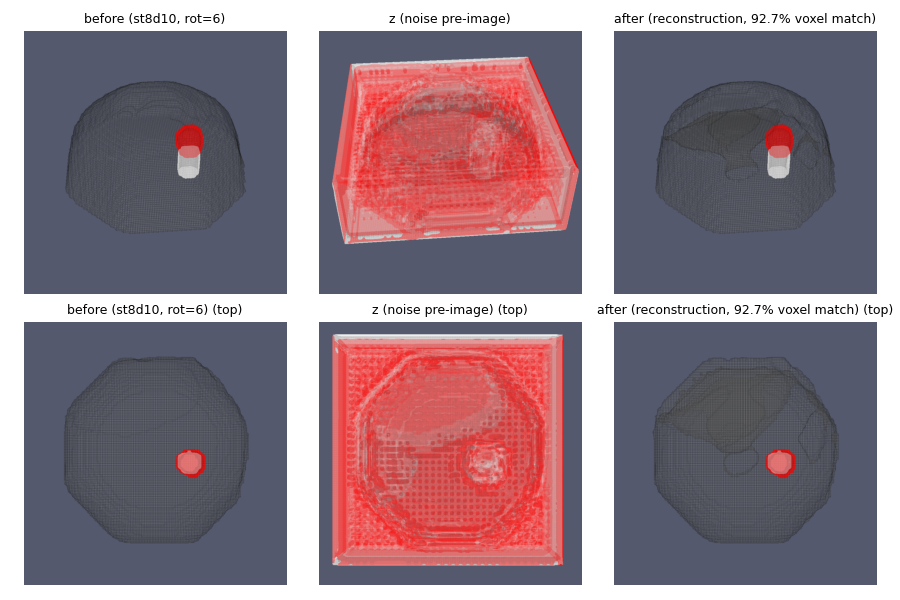
\includegraphics[width=\textwidth]{imgs/summary/inversion_example0.png}
    \caption{Before (real phantom) $\to$ $z$ (inverted noise pre-image) $\to$ after
    (re-generated from $z$), default and top-down views. The noise pre-image renders as an
    oversized, boxy lump region because argmax'd near-Gaussian noise splits roughly evenly
    across the four channels, unlike real anatomy where background dominates.}
    \label{fig:inversion}
\end{figure}

\subsection{Results}
Interpolating between two \emph{different} real phantoms was unreliable. Two failure modes
recurred across pairs: the generated volume sometimes collapsed almost entirely onto one
endpoint rather than blending; in other cases the predicted lump centroid landed close to the
naively expected linear position, yet the surrounding anatomy itself visibly tore, growing
extra bumps and disconnected fragments not present in either endpoint
(Figure~\ref{fig:interp-broken}). Neither more training epochs, the class-weighted loss of
Eq.~\ref{eq:weighted-loss}, nor a $3\times$ increase in integration steps changed this pattern,
which rules out both undertraining and numerical discretization error as the cause.

\begin{figure}[H]
    \centering
    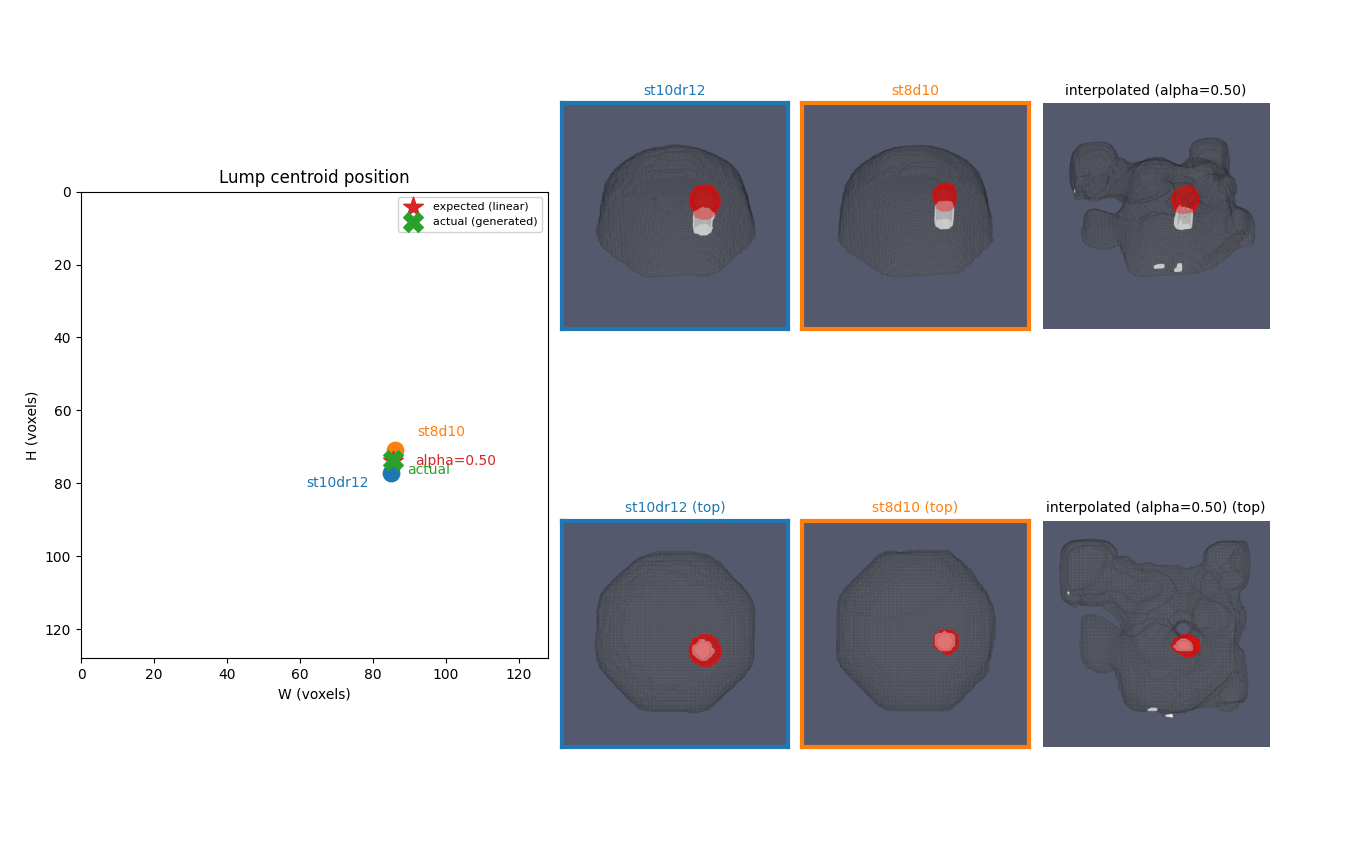
\includegraphics[width=\textwidth]{imgs/summary/interp_broken_example.png}
    \caption{A representative interpolation (pair \texttt{st10dr12}$\leftrightarrow$
    \texttt{st8d10}, $\alpha=0.5$). Left: the naively expected lump position (red star) versus
    what the model actually generated (green $\times$), close in this case. Right: renders of
    both endpoints and the interpolated result, showing extra bumps and disconnected specks
    absent from either endpoint.}
    \label{fig:interp-broken}
\end{figure}

\subsection{A partial-inversion variant ($t_{\text{mid}}$)}
Flow matching has no compression bottleneck: the noise space has the same dimension as the data
space, and nothing in the training objective (Eq.~\ref{eq:loss}) pushes it to be organized as a
whole. Training only ever supervises points that lie exactly on one phantom's own straight-line
path; with only $\sim10^3$ augmented training volumes scattered across a $\sim1.7\times10^6$
-dimensional space, the neighborhood \emph{between} two different phantoms' paths,
particularly near $t=0$, the least-constrained region of all, is never touched by training.
We tested a direct mitigation: rather than inverting each phantom all the way to $t=0$, invert
only \emph{partway} to an intermediate $t_{\text{mid}}>0$, interpolate the two partial
trajectories there, and integrate forward the remaining distance to $t=1$
(Figure~\ref{fig:tmid}). At larger $t_{\text{mid}}$ both trajectories are already pulled closer
to their own real anatomy, so the region between them is more likely to be one that real
training trajectories actually pass near.

\begin{figure}[H]
\centering
\resizebox{\textwidth}{!}{%
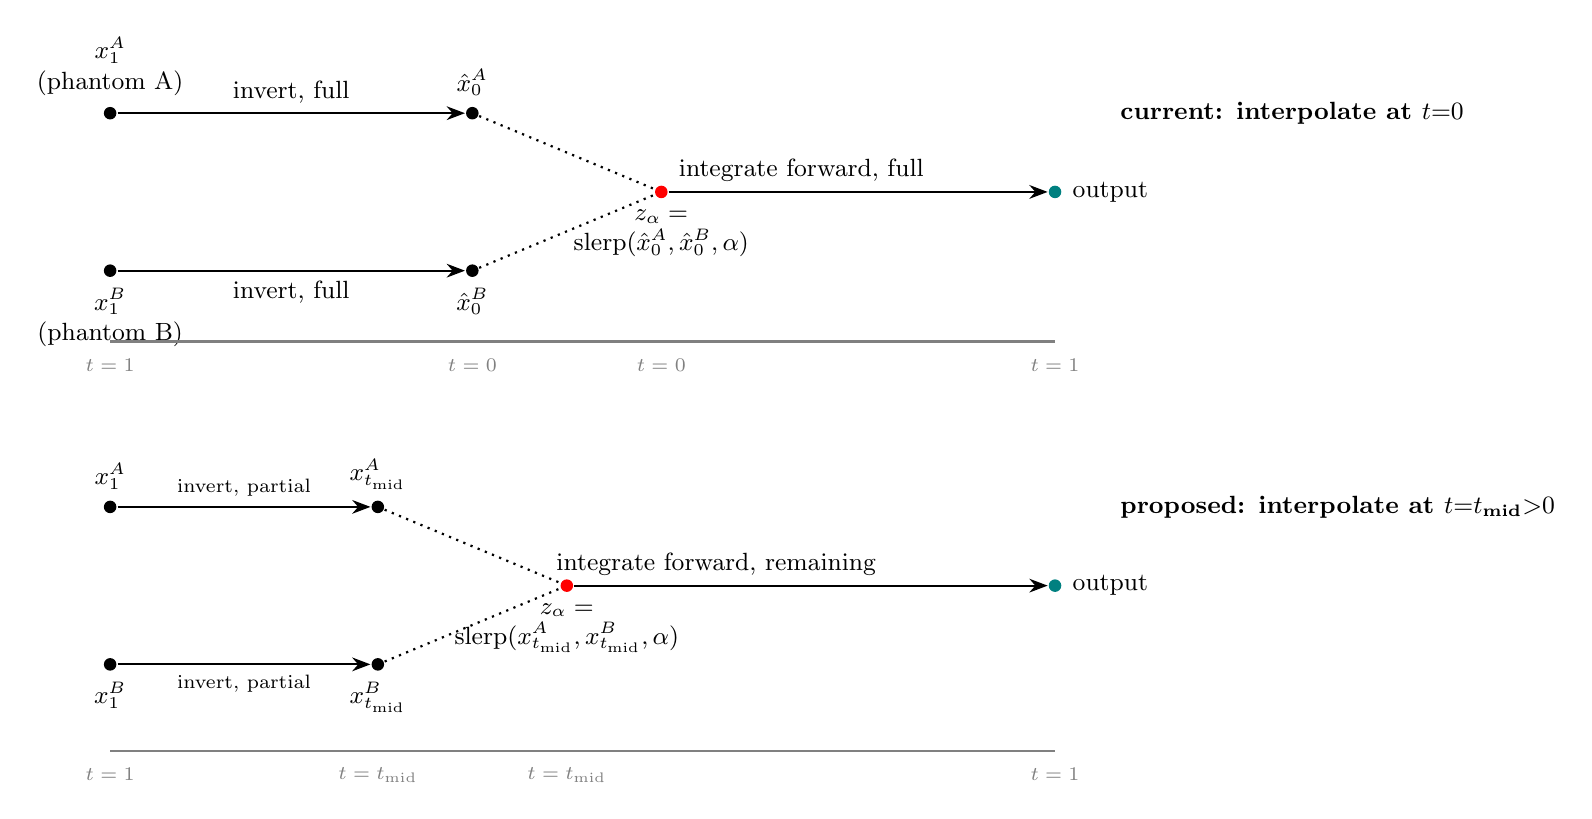
\begin{tikzpicture}[
  >=Stealth, thick,
  ptnode/.style={circle, fill, inner sep=1.6pt},
  every node/.style={font=\small}
]
\node[ptnode, label={[align=center]above:{$x_1^A$\\(phantom A)}}] (A1) at (0,3.2) {};
\node[ptnode, label={[align=center]below:{$x_1^B$\\(phantom B)}}] (B1) at (0,1.2) {};
\node[ptnode, label=above:{$\hat x_0^A$}] (A0) at (4.6,3.2) {};
\node[ptnode, label=below:{$\hat x_0^B$}] (B0) at (4.6,1.2) {};
\node[ptnode, fill=red, label={[align=center]below:{$z_\alpha =$\\$\mathrm{slerp}(\hat x_0^A, \hat x_0^B,\alpha)$}}] (Z1) at (7,2.2) {};
\node[ptnode, fill=teal, label=right:{output}] (O1) at (12,2.2) {};
\draw[->] (A1) -- node[above, pos=0.5]{invert, full} (A0);
\draw[->] (B1) -- node[below, pos=0.5]{invert, full} (B0);
\draw[dotted] (A0) -- (Z1);
\draw[dotted] (B0) -- (Z1);
\draw[->] (Z1) -- node[above, pos=0.35]{integrate forward, full} (O1);
\node[anchor=west] at (12.7,3.2) {\textbf{current: interpolate at $t{=}0$}};

\draw[-, gray] (0,0.3) -- (12,0.3);
\node[gray, font=\scriptsize] at (0,0.0) {$t=1$};
\node[gray, font=\scriptsize] at (4.6,0.0) {$t=0$};
\node[gray, font=\scriptsize] at (7,0.0) {$t=0$};
\node[gray, font=\scriptsize] at (12,0.0) {$t=1$};

\node[ptnode, label=above:{$x_1^A$}] (A1b) at (0,-1.8) {};
\node[ptnode, label=below:{$x_1^B$}] (B1b) at (0,-3.8) {};
\node[ptnode, label=above:{$x_{t_{\text{mid}}}^A$}] (A0b) at (3.4,-1.8) {};
\node[ptnode, label=below:{$x_{t_{\text{mid}}}^B$}] (B0b) at (3.4,-3.8) {};
\node[ptnode, fill=red, label={[align=center]below:{$z_\alpha =$\\$\mathrm{slerp}(x_{t_{\text{mid}}}^A, x_{t_{\text{mid}}}^B,\alpha)$}}] (Z2) at (5.8,-2.8) {};
\node[ptnode, fill=teal, label=right:{output}] (O2) at (12,-2.8) {};
\draw[->] (A1b) -- node[above, pos=0.5, font=\scriptsize]{invert, partial} (A0b);
\draw[->] (B1b) -- node[below, pos=0.5, font=\scriptsize]{invert, partial} (B0b);
\draw[dotted] (A0b) -- (Z2);
\draw[dotted] (B0b) -- (Z2);
\draw[->] (Z2) -- node[above, pos=0.3]{integrate forward, remaining} (O2);
\node[anchor=west] at (12.7,-1.8) {\textbf{proposed: interpolate at $t{=}t_{\text{mid}}{>}0$}};

\draw[-, gray] (0,-4.9) -- (12,-4.9);
\node[gray, font=\scriptsize] at (0,-5.2) {$t=1$};
\node[gray, font=\scriptsize] at (3.4,-5.2) {$t=t_{\text{mid}}$};
\node[gray, font=\scriptsize] at (5.8,-5.2) {$t=t_{\text{mid}}$};
\node[gray, font=\scriptsize] at (12,-5.2) {$t=1$};
\end{tikzpicture}%
}
\caption{Both rows invert A, invert B, slerp, and integrate forward, the only difference is
how far back each phantom is inverted before interpolating. Both A and B are still inverted
independently and symmetrically; the proposal only stops the backward integration early.}
\label{fig:tmid}
\end{figure}

\subsection{Evaluation metrics}
We use two families of metric, computed directly on the generated label volume. \textbf{Centroid
MAE} compares, for a pair $(A,B)$ at mixing fraction $\alpha$, the naively expected lump position
$p_{\text{expected}}(\alpha) = (1-\alpha)p_A + \alpha p_B$ against the actual centroid of the
generated lump, averaged over all pair-$\alpha$ combinations. \textbf{Component counts} apply 3D
connected-component labeling to the generated foreground and lump masks; real phantoms have
exactly one connected lump component and four connected anatomy components, so these are the
target values and larger counts indicate torn, fragmented anatomy.

\subsection{$t_{\text{mid}}$ results and analysis}
We swept $t_{\text{mid}}$ from $0.1$ to $0.9$ on 20 real-phantom pairs $\times$ 3 mixing
fractions (Table~\ref{tab:tmid}). Taken at face value this looks like a real improvement:
centroid MAE drops by roughly 40\% from $t_{\text{mid}}=0.1$ to its plateau around
$0.6$--$0.7$, and anatomy fragmentation drops by more than $4\times$ over the same range.

\begin{table}[H]
\centering
\begin{tabular}{c c c c}
\toprule
$t_{\text{mid}}$ & centroid MAE (voxels) & avg.\ anatomy components & avg.\ lump components \\
\midrule
0.1 & 10.81 & 22.78 & 7.18 \\
0.2 & 7.93  & 25.82 & 5.32 \\
0.3 & 6.86  & 26.57 & 2.97 \\
0.4 & 6.80  & 23.50 & 2.23 \\
0.5 & 6.86  & 17.67 & 2.62 \\
0.6 & 6.55  & 7.73  & 3.12 \\
0.7 & 6.40  & 5.77  & 5.15 \\
0.8 & 7.10  & 5.07  & 3.78 \\
0.9 & 7.15  & 6.17  & 1.72 \\
\bottomrule
\end{tabular}
\caption{$t_{\text{mid}}$ sweep, averaged over 20 real-phantom pairs $\times$ 3 mixing
fractions.}
\label{tab:tmid}
\end{table}

Inspecting the rendered examples the sweep also logged told a different story than the
aggregate numbers. Figure~\ref{fig:tmid-snap} shows the same pair at $t_{\text{mid}}=0.5$: at
$\alpha=0.25$ the output is essentially identical to phantom A rather than a blend toward B; at
$\alpha=0.5$ it shows \emph{both} phantoms' lumps simultaneously rather than one lump in
between. This pattern held across multiple pairs and across $t_{\text{mid}}\in\{0.1,0.5,0.9\}$:
the model behaves like a nearest-neighbor selector in angle, reproducing whichever endpoint
$\alpha$ is closer to, rather than smoothly interpolating. The centroid and fragmentation gains
in Table~\ref{tab:tmid} measure "looks closer to one real endpoint, less torn than a full
inversion" rather than "genuinely interpolates between the two."

\begin{figure}[H]
\centering
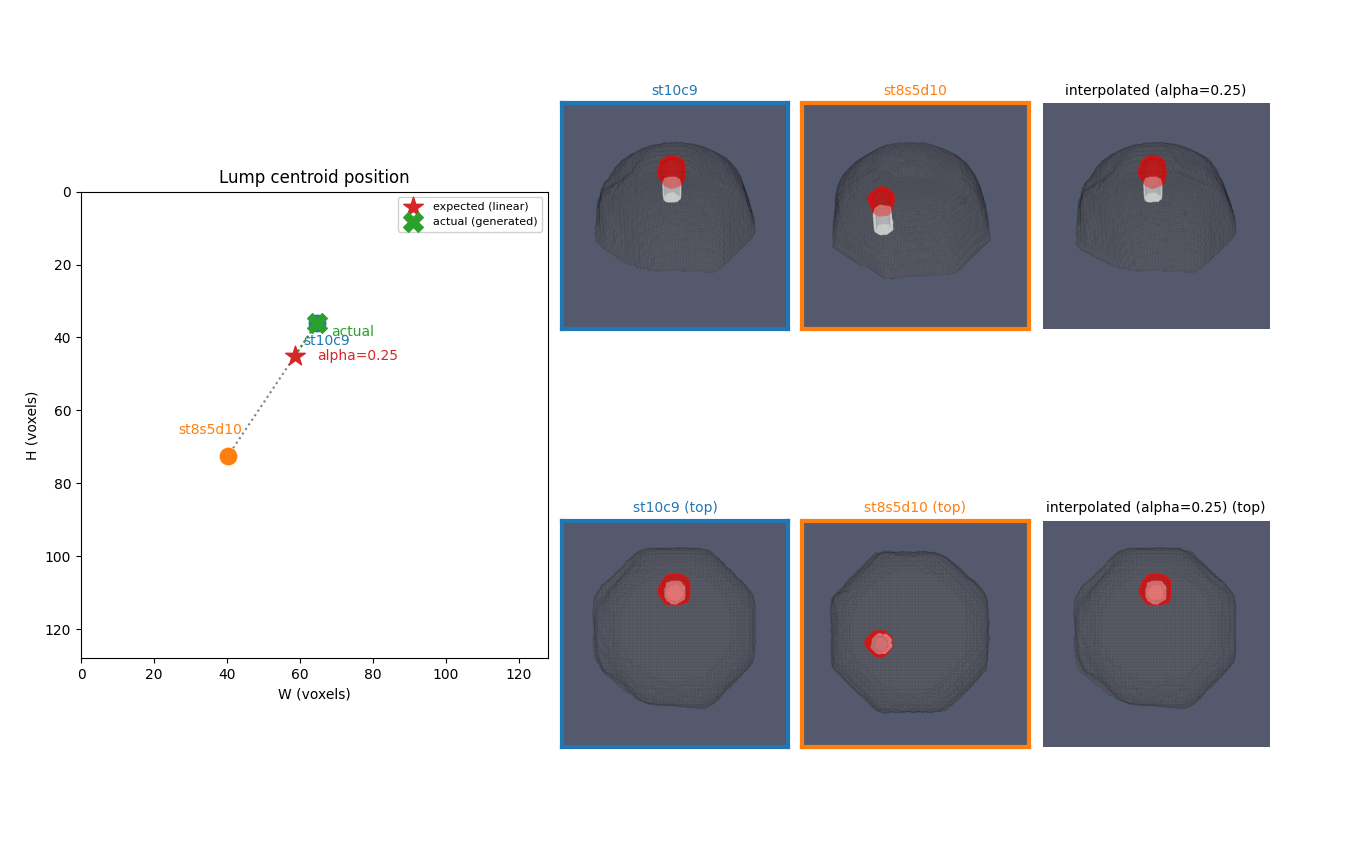
\includegraphics[width=0.48\textwidth]{imgs/summary/tmid_snap_alpha025.png}
\hfill
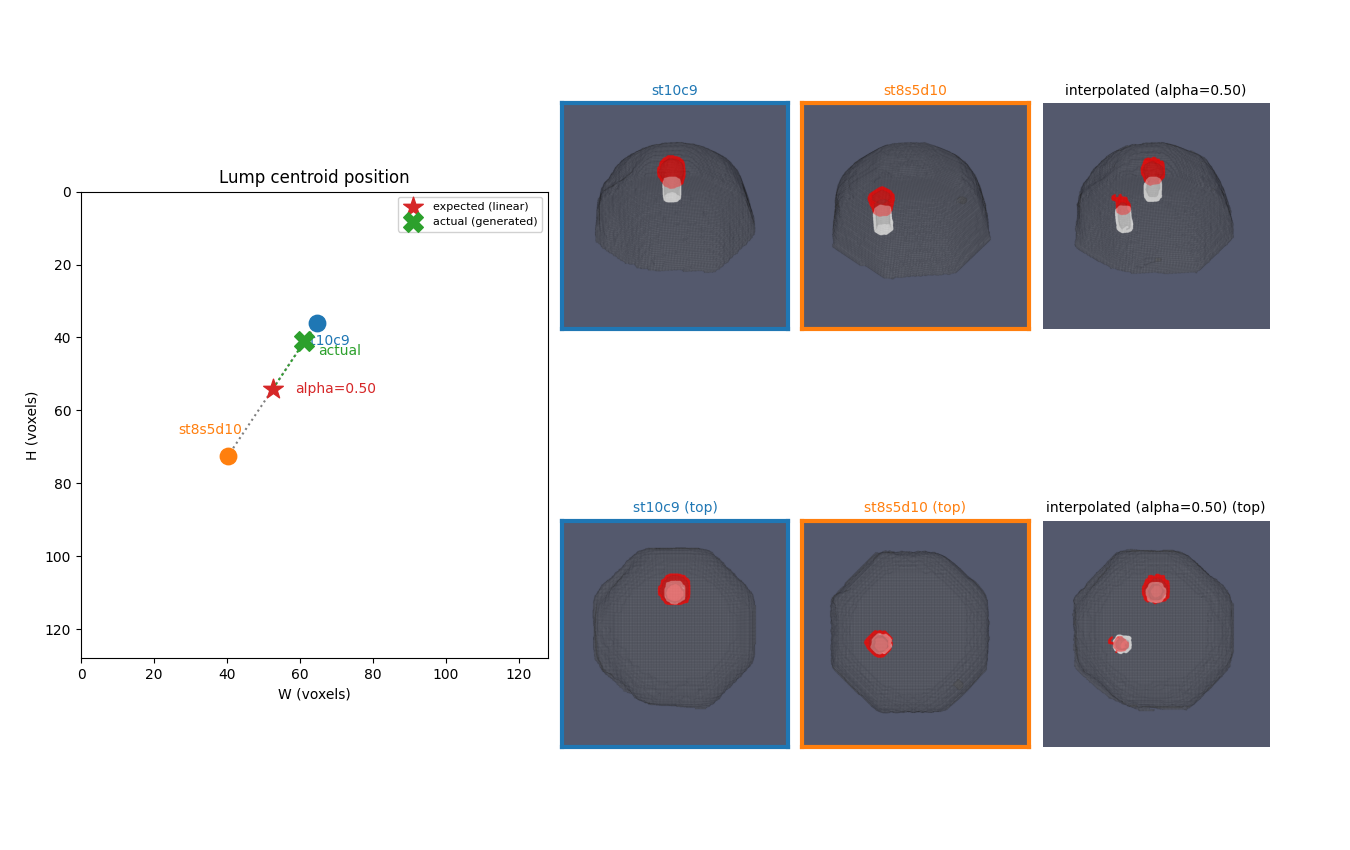
\includegraphics[width=0.48\textwidth]{imgs/summary/tmid_snap_alpha050.png}
\caption{Same pair (\texttt{st10c9}$\leftrightarrow$\texttt{st8s5d10}), $t_{\text{mid}}=0.5$.
Left, $\alpha=0.25$: output matches phantom A almost exactly. Right, $\alpha=0.5$: both A's and
B's lumps appear simultaneously instead of one blended lump.}
\label{fig:tmid-snap}
\end{figure}

\subsection{Summary}
The network was only ever taught the translation from noise-space position to anatomy \emph{at}
each individual real phantom's own inverted point; nothing in training ever supervised the
region between two different phantoms' points, at any $t_{\text{mid}}$. This is a structural
consequence of flow matching having no compression bottleneck, not a fixable bug in the
interpolation procedure itself, so we set the interpolation goal aside and looked for a task
that could give the model an exact, checkable target instead of one judged only by whether it
looks anatomically plausible.

\section{A Self-Supervised 180\textdegree{} Rotation Task}

\subsection{Task definition}
Every phantom is augmented with $8\times$ in-plane rotation at $45^\circ$ increments,
orientation $o\in\{0,\dots,7\}$. Because $180^\circ = 4\times45^\circ$, orientations $o$ and
$(o+4)\bmod 8$ of the same underlying phantom are an exact, bit-for-bit $180^\circ$ pair, giving
a task with a property interpolation never had: an exact, closed-form target for every input,
\begin{equation}
x_0 = \text{rotate}(x_{\text{raw}}, o), \qquad x_1 = \text{rotate}(x_{\text{raw}}, (o+4)\bmod
8). \label{eq:rotate180}
\end{equation}
Splitting phantoms by whether the lump sits right or left of the volume's vertical centerline
confirmed the framing geometrically: across all 984 augmented instances the split came out
exactly balanced (492/492) with zero ambiguous cases (Figure~\ref{fig:setsplit}), and every
$(o,o{+}4)$ pair lands on opposite sides by construction. Because $x_0$ is now always real data
rather than Gaussian noise, generation is a single forward integration (Eq.~\ref{eq:euler-fwd})
starting from the real $x_0$, so there is no inversion step, and no noise-space midpoint to be
inaccurate about.

\begin{figure}[H]
    \centering
    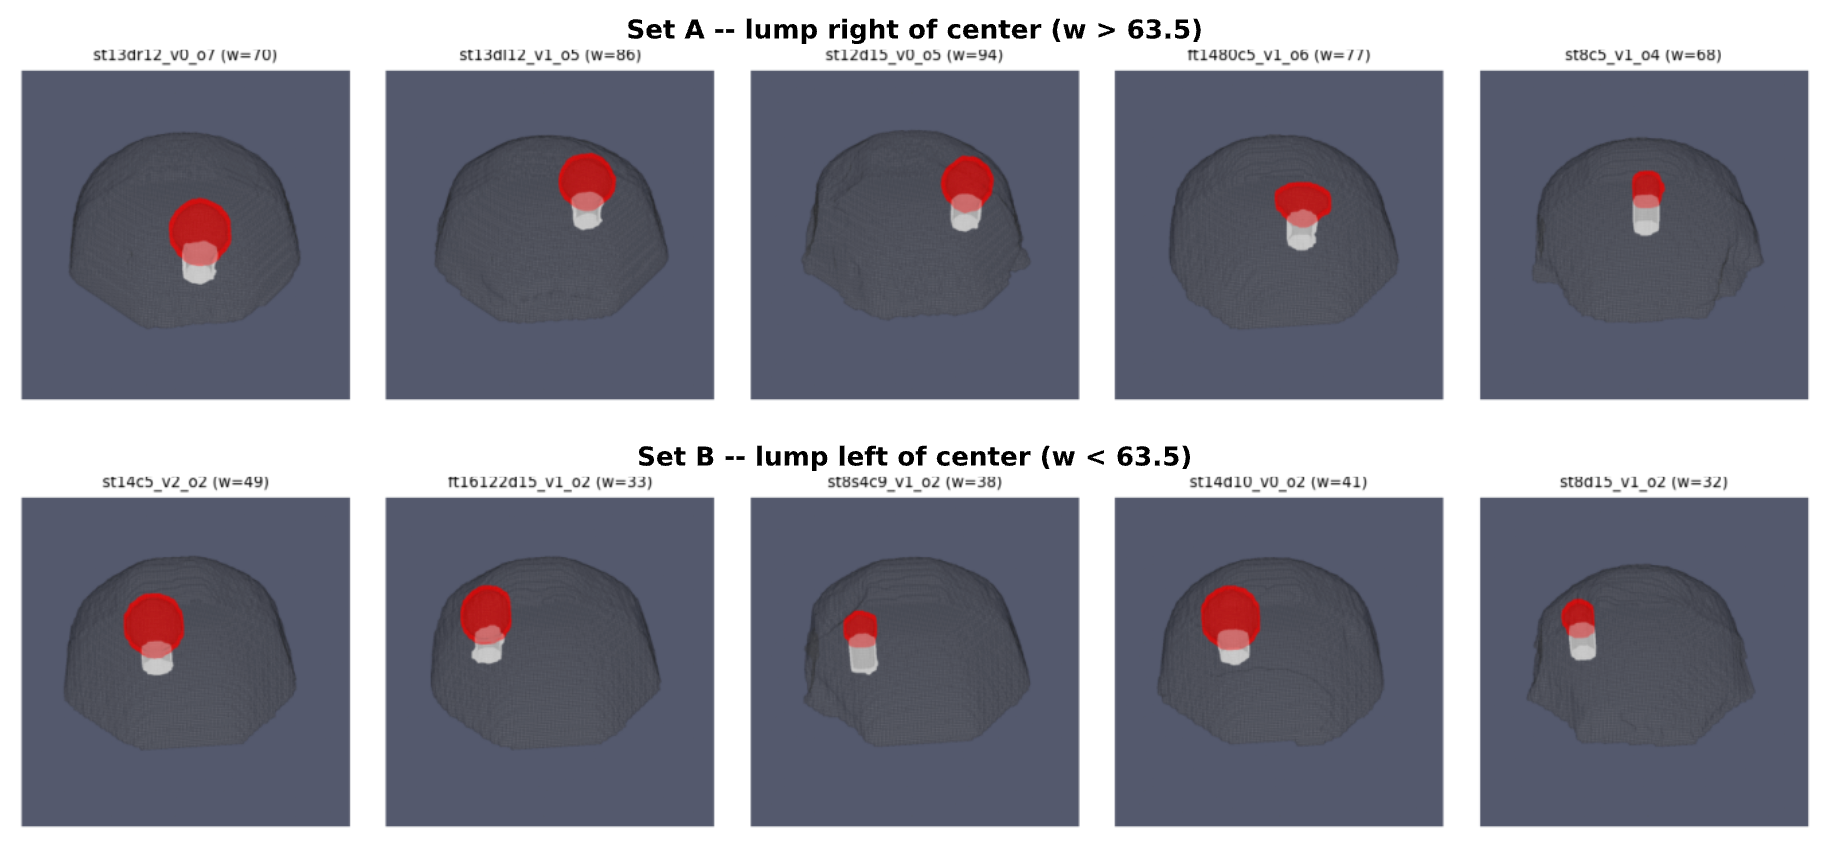
\includegraphics[width=\textwidth]{imgs/pres/setA_setB_split.png}
    \caption{Splitting all 984 augmented instances by lump position ($w\gtrless63.5$) gives an
    exactly balanced 492/492 partition with zero ambiguous cases, confirming that every
    $180^\circ$ pair connects opposite sides of the volume.}
    \label{fig:setsplit}
\end{figure}

\subsection{Baseline: velocity regression alone}
Training with the unweighted loss of Eq.~\ref{eq:loss} (now with $x_0$ real rather than noise)
produced a striking failure: \texttt{train/val\_loss} dropped substantially over hundreds of
epochs, yet the decoded prediction was voxel-for-voxel identical to $x_0$ on every tested
validation pair, unaffected by using up to $20\times$ more integration steps at inference.
Figure~\ref{fig:baseline} shows a representative example: the predicted lump centroid sits
directly on top of the original, far from the true $180^\circ$ target, yet gross voxel
agreement with the target is still 91.6\%, since background and insert dominate the volume closely
enough between the two orientations that a model which changes nothing at all can still score
deceptively well on a coarse, class-blind metric. This observation motivated the
class-sensitive, mask-based metrics used for the rest of this section. Separating the raw
velocity prediction's \emph{direction} from its \emph{magnitude} (checked against the exact
training-line target) showed the network already had a consistent directional signal
(cosine similarity $\approx0.65$); the predicted velocity magnitude was only about 20\% of what
was needed to actually flip a voxel's class after integration, an undercommitted regression
target, a typical symptom of plain MSE hedging once loss is already fairly low.

\begin{figure}[H]
    \centering
    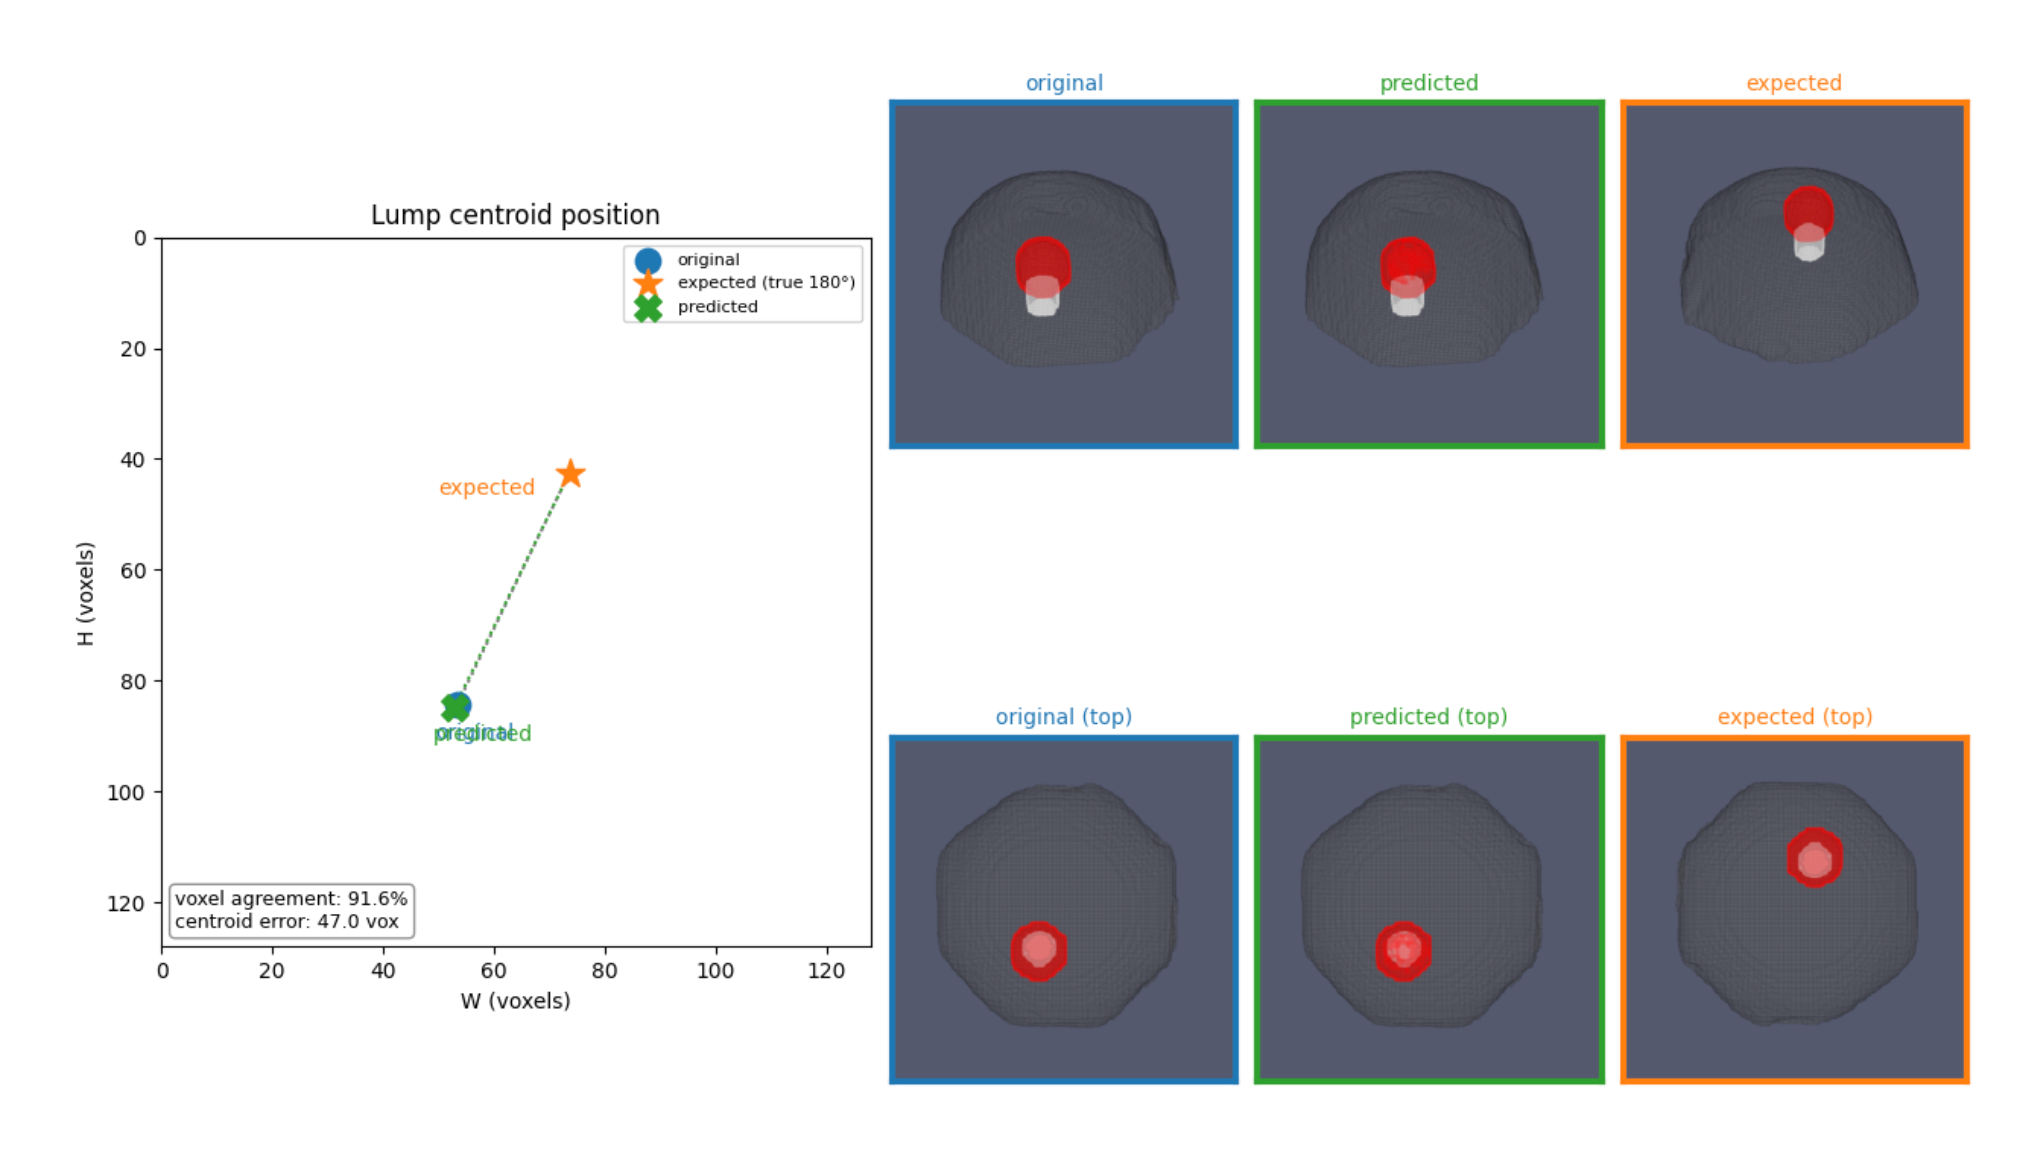
\includegraphics[width=\textwidth]{imgs/pres/baseline_no_move.png}
    \caption{Velocity-MSE-only baseline. The predicted lump position (green) coincides with the
    original (blue) rather than the true $180^\circ$ target (orange), despite 91.6\% gross
    voxel agreement with the target.}
    \label{fig:baseline}
\end{figure}

\subsection{A cross-entropy endpoint term}
Since $v^*=x_1-x_0$ is constant along the training line, algebra gives an endpoint estimate from
any point on the trajectory,
\begin{equation}
\hat x_1 = x_t + (1-t)\,v_\theta(x_t,t), \label{eq:endpoint}
\end{equation}
exact when $v_\theta=v^*$. Supervising this estimate with MSE against $x_1$ turns out to be an
exact reweighting of the existing velocity loss ($(\hat x_1-x_1)^2=(1-t)^2(v_\theta-v^*)^2$),
not a new training signal, so we used cross-entropy instead, whose gradient does not shrink as a
prediction approaches "good enough":
\begin{equation}
\mathcal{L}_{\text{pixel}} = \text{CE}\big(\hat x_1,\,\text{argmax}(x_1)\big), \qquad
\mathcal{L} = \mathcal{L}_{\text{velocity}} + \lambda_{\text{pixel}}\,\mathcal{L}_{\text{pixel}}.
\label{eq:pixel-loss}
\end{equation}
This directly countered the undercommitment: the decoded prediction started moving for the
first time, with a roughly 50--60\% reduction in lump-centroid distance within the first
$\sim$150 epochs. But it introduced a new failure mode: predictions became a massive, fragmented
mass covering much of the volume's cross-section (on the order of 24 disconnected lump
components versus about 1 on real phantoms), while centroid distance and gross voxel agreement
both stayed misleadingly reasonable, since a large blob's center of mass can coincidentally sit
near the true position. The root cause is specific to how class-weighted cross-entropy is
computed: the class weight is applied by each voxel's \emph{true} class, not its predicted one,
so missing a real lump voxel costs up to $12.57\times$ but wrongly predicting lump at a
true-background voxel costs only $1.0\times$, a direct incentive to over-predict the rare
classes wherever the network is unsure.

\subsection{Dice regularization, loss schedule, and EMA}
Three complementary changes addressed the over-prediction. A soft Dice term on the lump/pillar
channels penalizes false positives symmetrically with false negatives, unlike cross-entropy:
\begin{equation}
\mathcal{L}_{\text{dice}} = 1 - \frac{2\sum_v p_v t_v + 1}{\sum_v p_v + \sum_v t_v + 1}, \qquad
\mathcal{L} \mathrel{+}= \lambda_{\text{dice}}\,\mathcal{L}_{\text{dice}}. \label{eq:dice}
\end{equation}
The cross-entropy weight $\lambda_{\text{pixel}}$ was linearly decayed from $1.0$ to $0.3$ over
training, since held constant it sustained a $\sim$1.25--1.3$\times$ magnitude overshoot for
hundreds of epochs. An exponential moving average of the model weights (decay $0.999$) was used
for every evaluation and checkpoint, motivated by the aggregate lump-centroid error swinging
between roughly 17 and 60 voxels from one 25-epoch checkpoint to the next with no clear trend.
This combination fixed the gross over-prediction: predicted lump component counts fell from
the 20--60 range to mostly 2--14, but, as the next section shows, mask overlap with the true
target remained low.

\subsection{Evaluation metric: mask overlap}
Directly computing the Dice coefficient between the predicted and true binary lump mask,
\begin{equation}
\mathrm{Dice} = \frac{2|A\cap B|}{|A|+|B|},
\end{equation}
gave a mean of only $\approx0.13$ across ten validation pairs after adding the Dice term, decay
schedule, and EMA, nonzero and therefore meaningful, since the two positions are always
$180^\circ$ apart and can never overlap by chance, but far from good. A small blob that happens
to contain one true voxel can score near-zero overlap while its centroid looks correct, which is
exactly why mask overlap (not centroid distance) is used as the trusted metric throughout the
remainder of this section.

\subsection{Diagnosis: exposure bias, not numerical error}
Before revisiting the loss again, we tested whether integration accuracy was the bottleneck:
switching the sampler from Euler to Heun's method, and separately tripling the step count from
30 to 100, both left mean combined mask overlap essentially unchanged. This
rules out discretization error and points to \emph{exposure bias}: the network is only ever
trained at points exactly on the straight line between a real $(x_0,x_1)$ pair, so it fits that
narrow, teacher-forced objective well, but at inference it must integrate its own predicted
velocity forward, and small errors compound as its self-directed trajectory departs from that
line almost immediately.

\subsection{A rollout-consistency loss}
Every loss used so far is computed at a state constructed directly from the known pair
$(x_0,x_1)$, a question with an always-correct answer sitting in the data. At inference,
after the first step, the network instead faces a state \emph{it produced itself}, one it never
trained on. Rollout loss closes this gap by training on exactly the states the network's own
multi-step process produces: a short, gradient-tracked rollout from $x_0$ using the model's own
output at each step,
\begin{equation}
x^{(0)}=x_0, \qquad x^{(i+1)} = x^{(i)} + v_\theta\big(x^{(i)}, i\Delta t\big)\Delta t, \quad
i=0,\dots,k-1,\quad \Delta t = t_{\text{end}}/k, \label{eq:rollout}
\end{equation}
followed by the same endpoint-estimate cross-entropy and Dice terms (Eqs.~\ref{eq:pixel-loss},
\ref{eq:dice}) evaluated at the rolled-out state instead of a point on the true line. This
directly penalizes the drift responsible for exposure bias, at the cost of $k$ forward/backward
passes per training step with the full computation graph kept live. Applied to a
freshly-initialized network this proved unstable (predicted lump components on a from-scratch
run grew across the first three epochs rather than settling down); applied as a
\emph{continuation} of an already-competent checkpoint it was stable and produced real,
sustained improvement.

\subsection{Final checkpoint selection and validated results}
Every checkpoint saved by the rollout fine-tune was scored under identical conditions on 50
held-out pairs (Table~\ref{tab:checkpoints}). EMA weights beat raw weights at epoch 1250 but
\emph{lose} to raw weights at epoch 1500: the smoothing that helps mid-run becomes a liability
once the underlying weights have drifted past their best point. More importantly, training
longer did not help: the additional 250 epochs made every EMA metric worse, and only
partially recovered it for raw weights. Epoch 1250 (EMA) is the best model this run produced,
not the final one.

\begin{table}[H]
\centering
\begin{tabular}{@{}lcccc@{}}
\toprule
Checkpoint & lump Dice & pillar Dice & combined Dice \\
\midrule
epoch 1250 (raw) & 0.451 & 0.153 & 0.422 \\
\textbf{epoch 1250 (EMA)} & \textbf{0.498} & \textbf{0.268} & \textbf{0.478} \\
epoch 1500 (raw) & 0.470 & 0.262 & 0.448 \\
epoch 1500 (EMA) & 0.381 & 0.120 & 0.354 \\
\bottomrule
\end{tabular}
\caption{Every checkpoint saved by the rollout fine-tune, scored on the same 50 validation
pairs.}
\label{tab:checkpoints}
\end{table}

Running the full evaluation on epoch 1250 (EMA) across all 176 held-out validation pairs, plus a
matched sample of 176 training pairs, gives Table~\ref{tab:final}. Validation Dice is not lower
than train Dice, ruling out overfitting as an explanation for the result.
Figure~\ref{fig:final-traj} shows the full $t{=}0\to1$ trajectory for two held-out pairs: the
lump visibly separates from its starting position early in the integration and settles close to
its true $180^\circ$ target, with a clean, compact predicted shape rather than the diffuse
multi-component blob produced by the cross-entropy-only model or the oversized mass seen at
later, overtrained checkpoints.

\begin{table}[H]
\centering
\begin{tabular}{@{}lccc@{}}
\toprule
Split & lump Dice (mean) & pillar Dice (mean) & combined Dice (mean $\pm$ std) \\
\midrule
Validation (176 pairs) & 0.472 & 0.267 & $0.453 \pm 0.151$ \\
Train (176 pairs) & 0.429 & 0.247 & $0.405 \pm 0.203$ \\
\bottomrule
\end{tabular}
\caption{Final checkpoint (epoch 1250, EMA), full-dataset evaluation.}
\label{tab:final}
\end{table}

\begin{figure}[H]
\centering
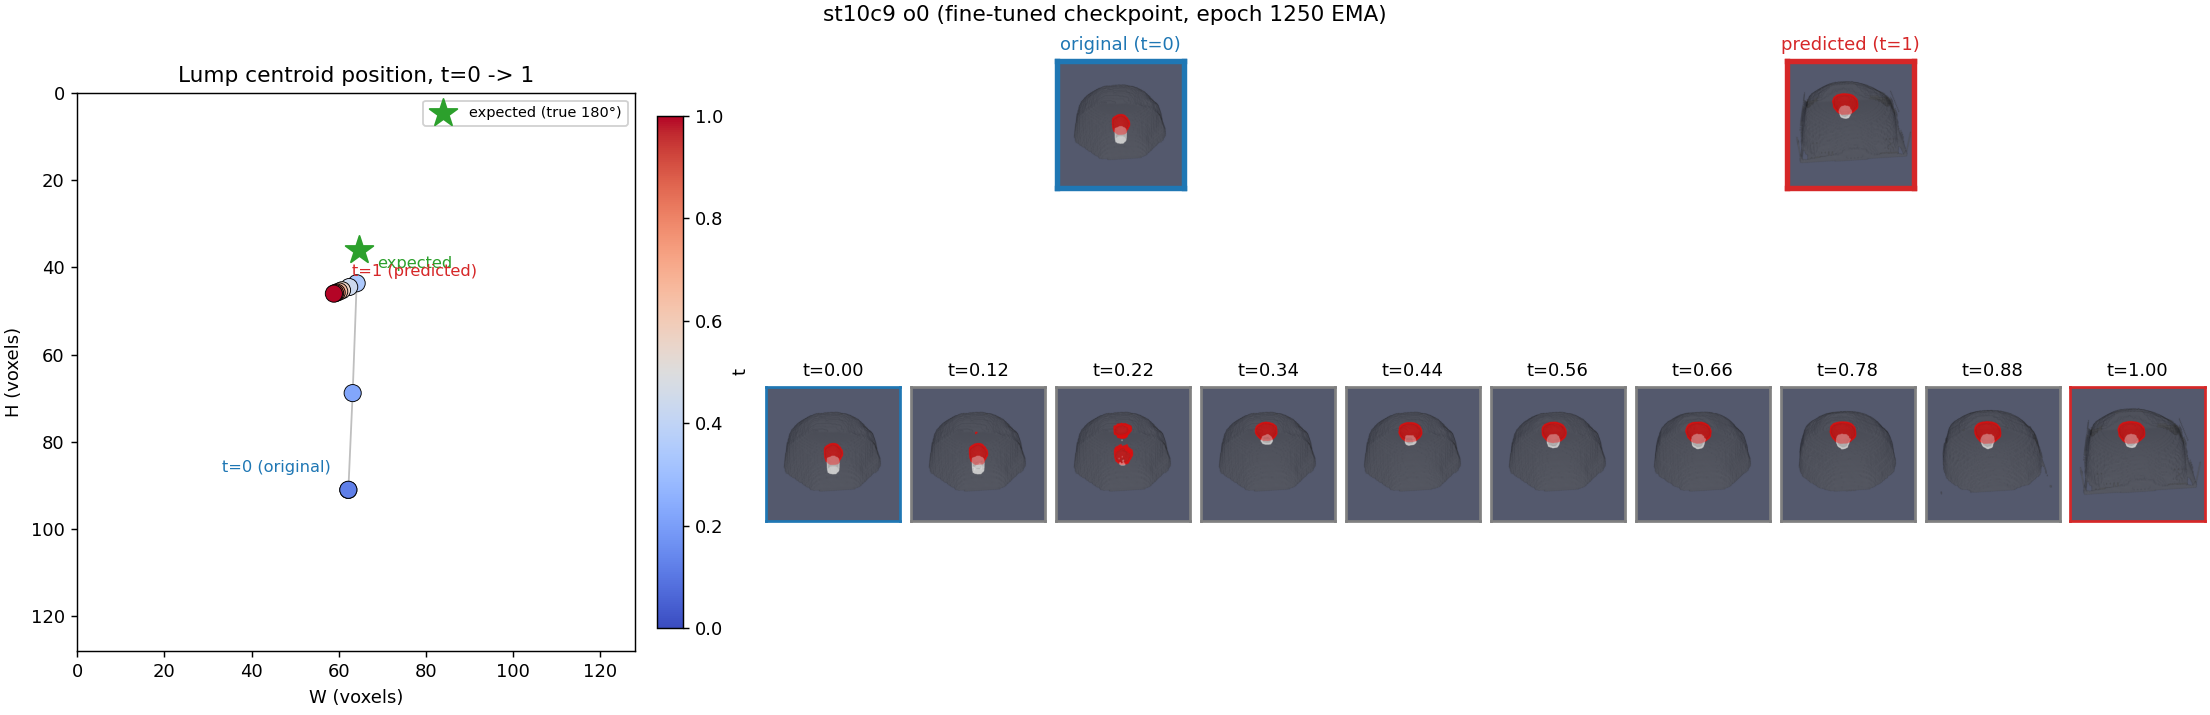
\includegraphics[width=\textwidth]{imgs/summary/rollout_trajectory_st10c9_o0.png}
\\[6pt]
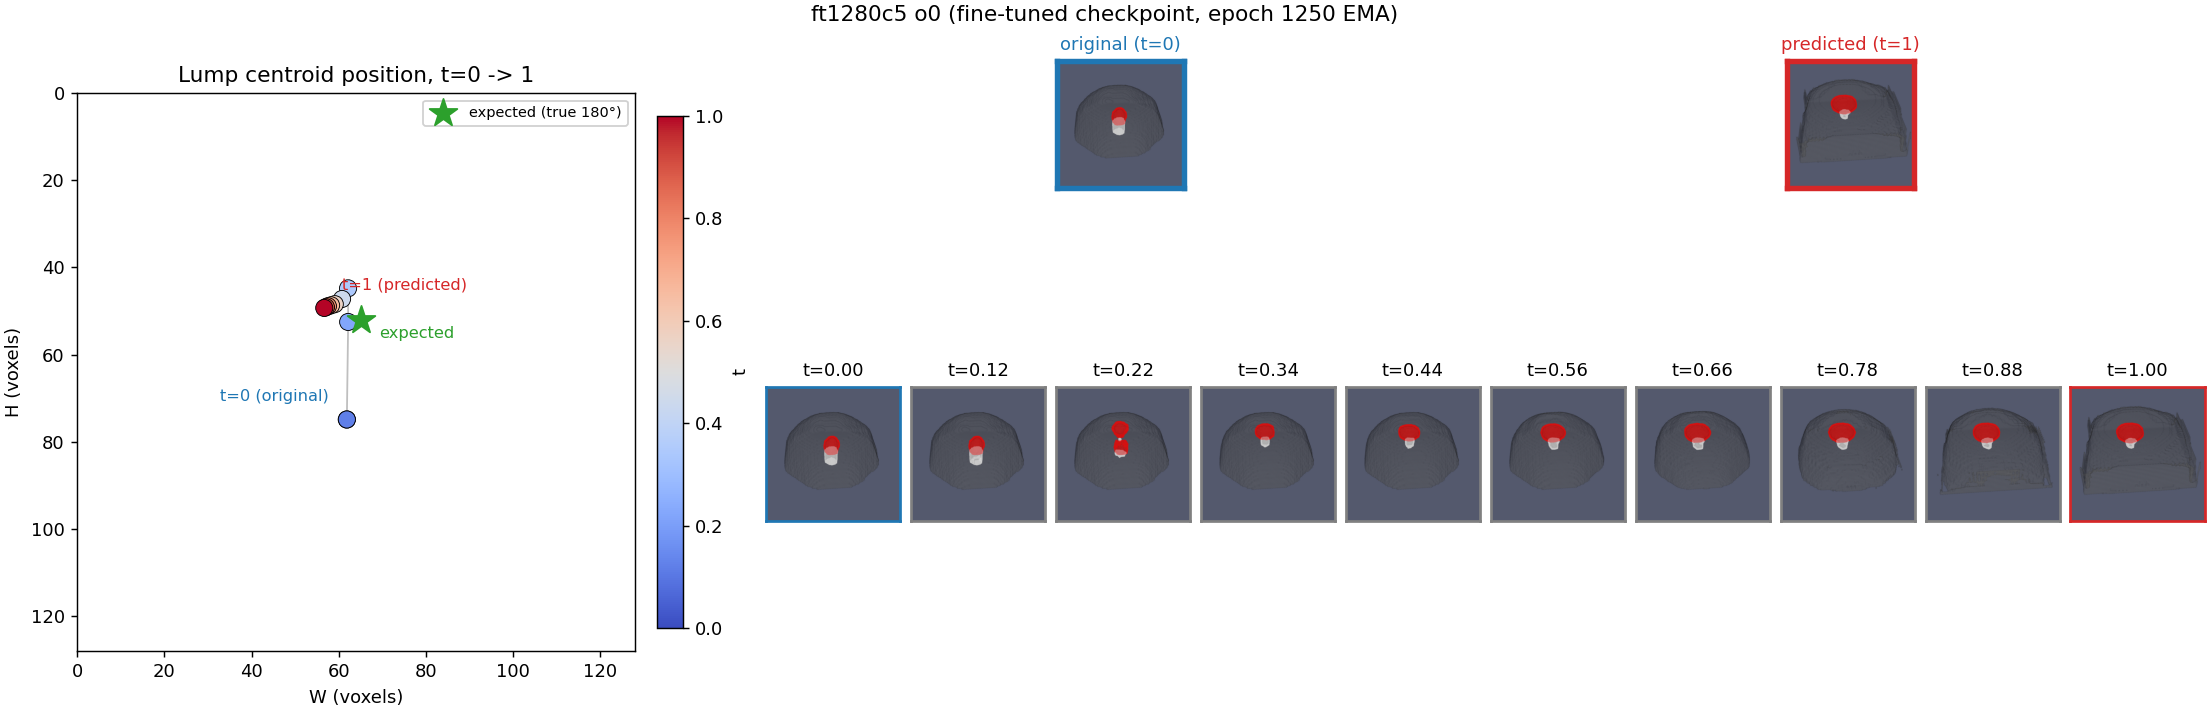
\includegraphics[width=\textwidth]{imgs/summary/rollout_trajectory_ft1280c5_o0.png}
\caption{Full $t{=}0\to1$ trajectory for the final checkpoint on two held-out validation pairs.
Left: the lump centroid's path through the volume, color-graded by $t$, against the true
$180^\circ$ target (green star). Right: original phantom, intermediate integration steps, and
final prediction.}
\label{fig:final-traj}
\end{figure}

\section{Conclusion}
Interpolating between real phantoms by inverting to noise, blending, and integrating forward did
not work on this dataset, and the failure persisted across more training, a class-weighted loss,
more integration steps, and a partial-inversion variant, because nothing in flow matching's
training objective constrains the region between two different real phantoms' noise
representations. Reformulating the problem as a self-supervised $180^\circ$ rotation task, which
supplies an exact target for every prediction, made the failure tractable: diagnosing an
undercommitted velocity field, an over-permissive cross-entropy term, and finally exposure bias
between teacher-forced training and the model's own multi-step rollout led to a
rollout-consistency loss that took the task from a model that never moves its prediction at all
to one that reliably relocates the lump to its true target, with a validated combined Dice of
$0.453 \pm 0.151$ on 176 held-out pairs and no indication of overfitting to the training set.

\end{document}
